\section{Definition}\label{s:definition}
Derzeit gibt es keine passende Definition, die den Begriff Robotik bzw. mobile Roboter so präzise formuliert, dass sie auf genau die Objekte passt, die nach gemeingültigen Kriterien einen Roboter definieren \cite{hertzberg2009mobile}. In \cite{hertzberg2009mobile} erklärt der Autor, dass es nicht unüblich ist, dass diese Unschärfe in der Definition großartig stört. Eine allgemeine Definition für Robotik ist in der \ac{VDI} Richtlinie 2860 von 1990 zu finden:
\\
\\
\textit{"`Ein Roboter ist ein frei und wiederprogrammierbarer, multifunktionaler Manipulator mit mindestens drei unabhängigen Achsen, um Materialien, Teile, Werkzeuge oder spezielle Geräte auf programmierten,
variablen Bahnen zu bewegen zur Erfüllung der verschiedensten Aufgaben."'}
\\
\\
Allerdings passt diese Definition nicht gut auf mobile Roboter. Diese Sprachregelung der \ac{VDI} zielt eher auf Handhabungsroboter aus der Automatisierungstechnik oder auf Kommissionierroboter aus dem Logistik-Bereich ab. Gemeint sind damit sogenannte \textit{stationäre Robotersysteme} \cite{Haun2007}. Diese sind starr mit der Umgebung verbunden und besitzen einen festgelegten Arbeitsraum. Damit sind die oben genannten "`programmierten, variablen Bahnen"' möglich, da der Arbeitsprozess in dem sich der Roboter befindet vorher bekannt ist und dadurch programmierbar wird. 

Mobile Robotersysteme unterscheiden sich zu stationären grundlegend, indem sie ihre Position durch Lokomotion (aus eigener Kraft) verändern \cite{Haun2007}. Somit hängen alle ihre Aktionen direkt von ihrer aktuellen Umgebung ab, die detailliert immer erst zum Zeitpunkt der Ausführung bekannt wird \cite{hertzberg2009mobile}. Sowohl \cite{hertzberg2009mobile} als auch \cite{Haun2007} heben die Eigenschaft hervor, dass mobile Roboter ihre Umgebung mittels Sensoren (vgl. Kapitel \myref{Komponenten} erfassen und auswerten müssen. Aus dem Ergebnis der Auswertung wählen sie schließlich ihre nächste Aktion. Ferner werden in \cite{Haun2007} folgende, weitere Eigenschaften genannt:
\begin{itemize}
\item Aufgabenorientierte und implizierte Programmierung,
\item Anpassung an Veränderungen an die Umgebung,
\item Lernen aus Erfahrungen und entsprechende Verhaltensmodifikation,
\item Entwicklung eines internen Weltbildes und
\item Manipulation physikalischer Objekte in der realen Welt
\end{itemize}
Das bedeutet im Allgemeinen, dass ein mobiler Roboter in einer zuvor nicht bekannten und nicht kontrollierbaren Umwelt zu jeder Situation abhängig der Umgebung operieren muss. Im Vergleich zu stationären Robotern bedeutet das nicht, dass die mobilen Roboter regellos oder zufällig arbeiten. Die entsprechenden Anweisungen sind "`weicher"', wie zum Beispiel eine Bahnplanung eines Industrieroboters.

Mit welchen internen und externen Sensoren ein Roboter seine Umgebung verarbeitet, wird in Kapitel \myref{Komponenten} erklärt.


\subsection{Roboterarten}
\textbf{Serviceroboter} sind Maschinen, die den Menschen bei der täglichen Arbeit unterstützen sollen. Darüber hinaus sollen sie auch in der Lage sein als Unterhaltungssystem zu dienen. Es wird geschätzt, dass in ca. 30 Jahren mehr persönliche Roboter produziert werden als persönliche Computer \cite{Haun2007}.
Diese sollten am Besten auf Zuruf alltägliche Arbeit erledigen können. Dazu zählt Staub saugen, Rasen mähen oder auch Fenster putzen. Dabei tritt häufig ein zentrales Problem in den Vordergrund: die Anatomie des Menschen. Diese ist ein regelrechtes Wunderwerk, da beispielsweise die menschliche Hand bei einem durchschnittlichen Gewicht von 600 Gramm und 23 verschiedenen Freiheitsgraden dazu in der Lage ist, Bewegungen mit stufenlos verstellbarer Feinfühligkeit durchzuführen. Vor allem japanische Forscher stecken viel Arbeit in die Erforschung immer besser werdender Serviceroboter. Der durch Honda im Jahr 2001 vorgestellte Serviceroboter \textit{Asimo} ist bei einer Größe von 1.20 Meter nur noch 43kg schwer (Siehe Abbildung \ref{f:asimo}).
Dabei ist eine der größten Herausforderungen die Stromversorgung. Ein Roboter, der ständig am Ladegerät hängen muss, hilft dem Menschen nicht weiter. Daraus resultiert, dass kommerzielle Anbieter von Staubsaugrobotern Räder als Antrieb benutzen. Diese Roboter müssen ihre Bewegungen nicht ständig korrigieren und fahren in konstanter Bodennähe durch die Gegend. Ferner ist die Interaktion zwischen Roboter und Mensch ein Problem. Das Robotersystem muss Daten nicht nur messen und analysieren, sondern auch bewerten können. Dabei gibt es immer noch keine geeignete Verarbeitung der intuitiven Kommunikation, die beim Menschen über Gestik, Mimik und Sprache erfolgt. So wird es noch einige Jahre dauern, bis Serviceroboter uns wirklich im Alltag unterstützen können.
\begin{figure}[H]						
	\centering							
	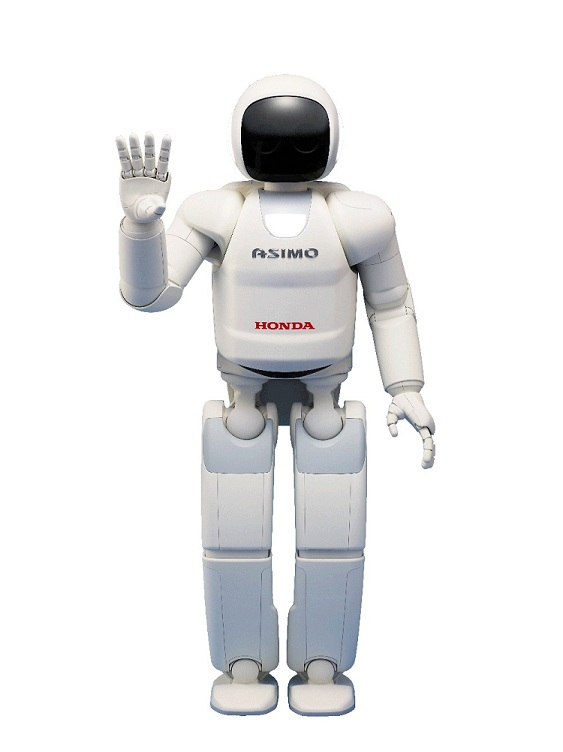
\includegraphics[scale=0.5]{Bilder/asimo.jpg}			
	\caption{Roboter ASIMO}						
	\label{f:asimo}						
\end{figure}

\textbf{Industrieroboter} hingegen haben sich in der aktuellen Zeit schon sehr etabliert. Der Autobauer Volkswagen setzt an einen Produktionsstandort ca. 760 Industrieroboter ein und insgesamt in Deutschland sind es sogar mehr als 100.000 Stück \cite{Haun2007}. Im Gegensatz zu den Servicerobotern haben sie meist nur einen Arm und besitzen keine Beine und keinen Kopf. Ihre Aufgabe besteht darin, selbst tonnenschwere Lasten zu heben und pausenlos gefährliche Arbeit wie das Schweißen durchzuführen. 
Theoretisch kann jedes Fertigungsproblem heutzutage auch maschinell gelöst werden. In der Autoindustrie gibt es beispielsweise weite Bereiche (Herstellung Karosserie), in denen Roboter dominieren. Dafür zeigt sich jedoch, dass diese in der Endmontage deutlich in der Minderheit liegen. Zukünftig sollen Industrieroboter ihre Befehle nicht mehr über eine grafische Benutzeroberfläche erhalten, stattdessen sollen sie ihre Aufgaben intuitiv per Sprachsteuerung erklärt bekommen\cite{Haun2007}.

Robotersysteme werden auch in Bereichen der \textbf{Medizin} eingesetzt. Durch ihre hohe Präzision fräsen sie beispielsweise Hüftgelenke so exakt aus, dass die Ersatzteile nahtlos und ohne Zement eingefügt werden können. Die Vorteile sind, dass sie frei von emotionalen Einflüssen sind und keine Tagesform kennen. Egal zu welchem Zeitpunkt, die programmierte Aufgabe erledigt der Roboter immer gleich. Allerdings sind sie teuer und kompliziert. Die Operation muss im Vorfeld genauestens geplant werden und auf sich plötzlich verändernde Gegebenheiten kann ein Roboter nicht reagieren. So musste unter anderem der \textit{Robodoc} abgeschaltet werden, da er Menschen Schaden zugefügt hat. Als Schlussfolgerung hat sich derzeit der Einsatz von Robotern in der Medizin eher auf die Form eines Assistenten reduziert. Die Maschine hält dabei Skalpell und Nadel und führt als verlängerter Arm aus, was der menschliche Operateur hinter dem Steuer vorgibt \cite{Haun2007}. Solche Systeme werden vor allem bei Herzoperationen eingesetzt, da sie jedes Zittern des Menschen herausfiltern und so an kleinsten Gefäßen und Strukturen arbeiten können. Die Roboter helfen dabei, schwierige Operationen zu vereinfachen.

\textbf{Humanoide Roboter} sind menschenähnliche Roboter, wie \textit{Asimo} (Abbildung \ref{f:asimo}) oder Nao. Ihr Bau ist nicht nur durch den Spieltrieb der Robotiker oder der Sensationslust des Publikums motiviert. Auch wissenschaftliche Aspekte sprechen für den Bau humanoider Roboter. So wird nur ein Roboter mit einem menschenähnlichen Körper auch menschenähnliche Begriffe und Denkweisen entwickeln \footnote{Johnson 1987}. Ferner spielt natürlich auch der psychologische Aspekt im Bereich der Servicerobotik eine Rolle. Wenn etwas wie ein Mensch aussieht, wird damit auch umgegangen wie mit einem Menschen. Einem humanoiden Roboter kann ein Mensch, wie seinem menschlichen Gegenüber, seine Wünsche mitteilen und braucht dafür keine Gebrauchsanweisung. Dazu kommt, dass ihre Körper auch auf die Umgebung abgestimmt sind, in der sich der Mensch bewegt.


